

\subsection{Cellular Network Architecture}

A cellular network is a wireless communication system that provides mobile devices with access to internet services and Mobile communication. To provide coverage over large geographical areas, network operators deploy base stations at different locations. Each base station serves users within its coverage area and together they can cover wide geographical areas. As shown in Figure \ref{fig:network_archetecture}, multiple base stations can be deployed to form a connected network covering a wide area. \\

\begin{figure}[h]
    \centering
    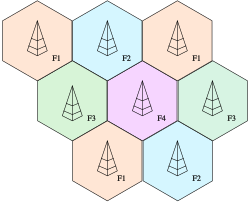
\includegraphics[width=\linewidth]{figures/Frequency_reuse.png}
    \caption{Cellular network architecture showing base stations, user devices, and inter-cell connectivity.}
    \label{fig:network_archetecture}
\end{figure}

Modern base stations are commonly divided into sectors covering approximately 120 degrees each \cite{120_degree_sectors}. Within each sector, multiple cells may operate on different frequency bands and technologies, such as 4G and 5G. A base station consist of multiple cells and the cell is the basic unit of the network and handles communication between user devices and the network. \\

User devices connect to the network by attaching to the cell that provides the best radio conditions. This decision is mainly based on signal strength and signal quality, which are continuously measured by the device and the network. One key metric is the signal-to-interference-plus-noise ratio (SINR), which describes the quality of the received signal relative to background noise and interference from neighboring cells. \\

As users move or radio conditions change, connections may be transferred between cells in a process called handover \cite{handoff}. Handover ensures continuous connectivity by moving the user to a cell with better signal quality or more available capacity when needed. \\



\subsection{Modulation and Signal Quality}
Orthogonal Frequency Division Multiplexing (OFDM) is a multi carrier modulation technique that divides a wide frequency band into many narrow, parallel subcarriers ~\cite{ofdm_paper}. Each subcarrier is shaped as a sinc function in the frequency domain, which produces a peak at its own center frequency and crosses zero at the center frequencies of all neighboring subcarriers as seen in figure \ref{fig:ofdm_sinc_function}. \\

This means that even though the subcarriers overlap in spectrum, sampling each one at its own center frequency yields no contribution from its neighbors, they are mathematically orthogonal. The subcarrier spacing is chosen carefully to be the inverse of the symbol duration, which guarantees these zero crossings align. This allows subcarriers to be packed far more tightly than traditional frequency division multiplexing, where guard bands would be required to prevent interference, resulting in much more efficient use of spectrum. \\

\begin{figure}[h]
    \centering
    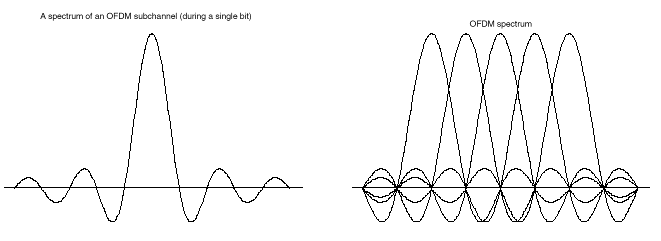
\includegraphics[width=\linewidth]{figures/ofdm.png}
    \caption{OFDM Sinc function alone vs with 5 subcariers}
    \label{fig:ofdm_sinc_function}
\end{figure}

%These subcarriers are grouped in the time-frequency domain into Physical Resource Blocks, forming the basic scheduling unit described in Section \ref{sec:prb}. The amount of data that can be carried by each resource block depends not only on how many blocks are allocated, but also on the modulation scheme applied to each subcarrier. \\

Modern cellular networks employ adaptive modulation schemes, where the modulation order is selected according to the user's radio conditions \cite{ericsson5gnr}. Quadrature Amplitude Modulation (QAM) encodes information by varying both the amplitude and phase of the transmitted signal. Each combination of amplitude and phase corresponds to a unique symbol in the constellation diagram shown in Figure \ref{fig:QAM_constallation_diagram}. \\

The number of bits carried by a symbol depends on the modulation order and can be expressed as

\[
b = \log_2(M)
\]

where M is the number of constellation points. Modulation schemes supported in LTE and NR systems include QPSK, 16QAM, 64QAM, and
256QAM in both uplink and downlink \cite{ericsson5gnr}, corresponding to 2, 4, 6, and 8 bits per symbol respectively.

%For example, QPSK (M=4) carries 2 bits per symbol, 16-QAM carries 4 bits per symbol and 64-QAM carries 6 bits per symbol. \\


\begin{figure}[H]
    \centering
    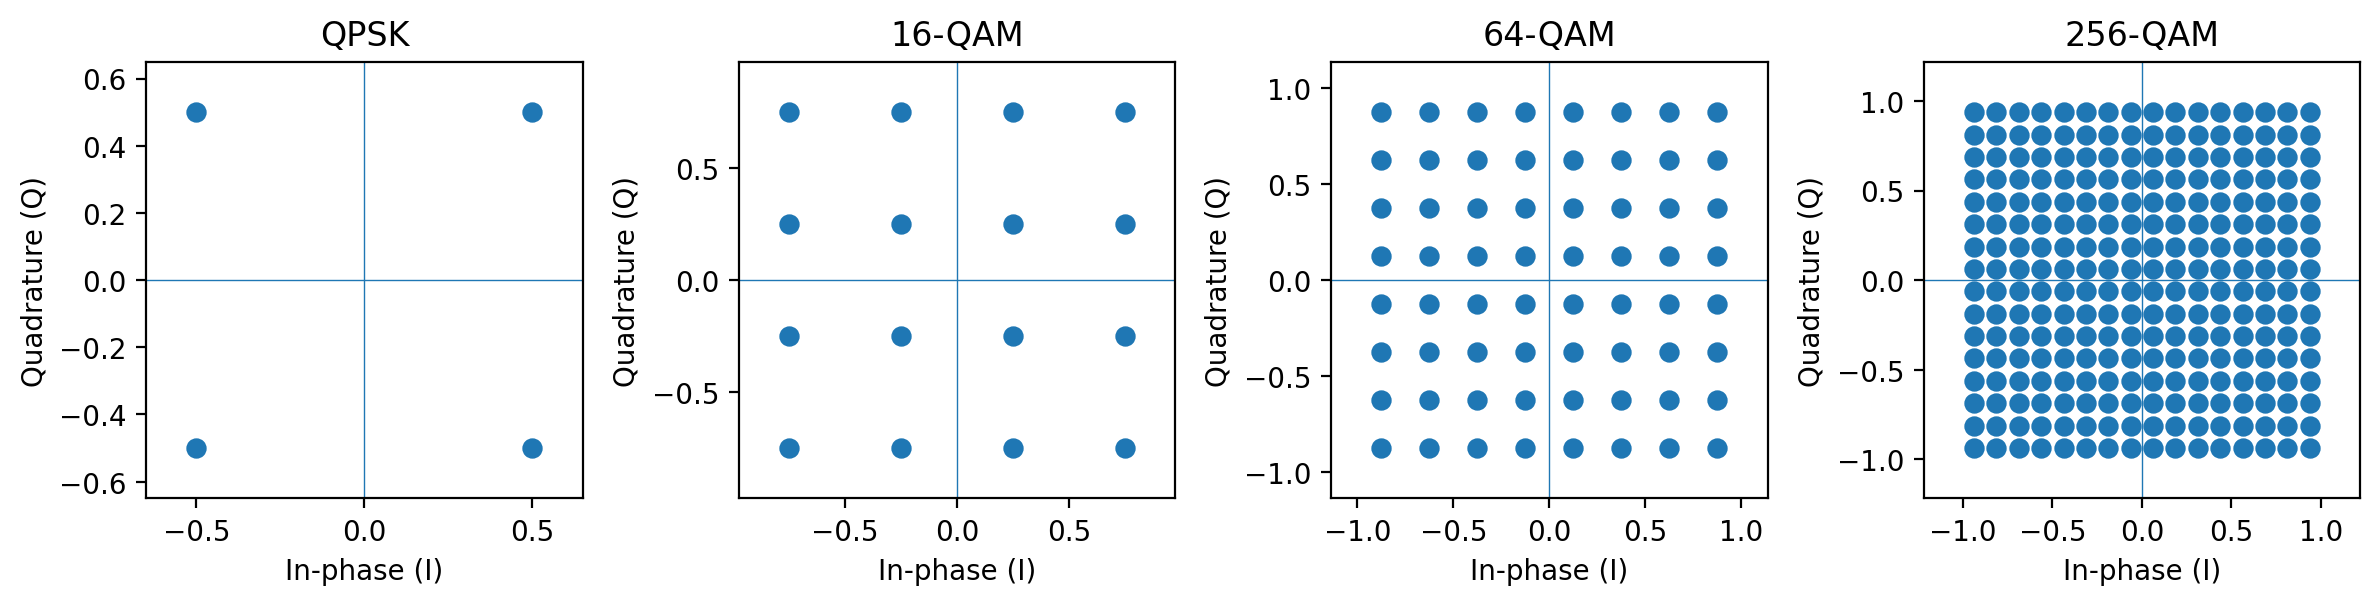
\includegraphics[width=\linewidth]{figures/qam_1_axis.png}
    \caption{Constellation diagrams for different modulation schemes, illustrating the increasing number of symbols and bits per symbol from QPSK to higher-order QAM.}
    \label{fig:QAM_constallation_diagram}
\end{figure}


%he modulation order selected by the scheduler depends on the radio conditions experienced by the user equipment, primarily expressed through the Signal-to-Interference-plus-Noise Ratio (SINR) or Channel Quality Indicator (CQI). Radio condition is influenced by several factors including distance to the base station, propagation conditions,interference from neighboring cells and the speed the user is moving at. As Radio conditions increases, constellation points can be placed closer together while still being reliably distinguished by the receiver, allowing higher-order modulation schemes to be used. Users experiencing bad radio conditions must fall back to lower-order schemes, which are more robust to noise but carry fewer bits per symbol. \\

The modulation order selected by the scheduler depends on the radio conditions experienced by the user equipment, primarily expressed through the Signal-to-Interference-plus-Noise Ratio (SINR) or Channel Quality Indicator (CQI). The base station performs link adaptation based on these measurements, selecting an appropriate Modulation and Coding Scheme (MCS) to match the current channel quality \cite{3gpp_ts38214}. As channel conditions improve, higher order modulation schemes can be used because constellation points can be placed closer together while remaining reliably distinguishable at the receiver. Conversely, under poor channel conditions, the system falls back to lower order modulation schemes, which are more robust to noise and interference but carry fewer bits per symbol. \\


The trade-off between modulation order and reliability can be quantified through the Bit Error Rate (BER). For square M-QAM, the theoretical BER as a function of the received $E_b/N_0$ is well approximated by:
\[
\text{BER} \approx \frac{4}{\log_2 M} \left(1 - \frac{1}{\sqrt{M}}\right) \text{Q}\!\left(\sqrt{\frac{3 \log_2 M}{2(M-1)} \cdot \frac{E_b}{N_0}}\right)
\]
where $M$ is the modulation order, $E_b/N_0$ is the energy per bit to noise power spectral density ratio, $\log_2(M)$ is the number of bits carried per symbol, and $Q(x)$ is the standard Gaussian Q-function, representing the probability that a standard normal random variable exceeds $x$. \\



Figure~\ref{fig:BER_plot}, higher-order modulation schemes require a significantly 
larger $E_b/N_0$ to achieve the same bit error rate, reflecting the reduced distance between 
constellation points in figure \ref{fig:QAM_constallation_diagram}

\begin{figure}[H]
    \centering
    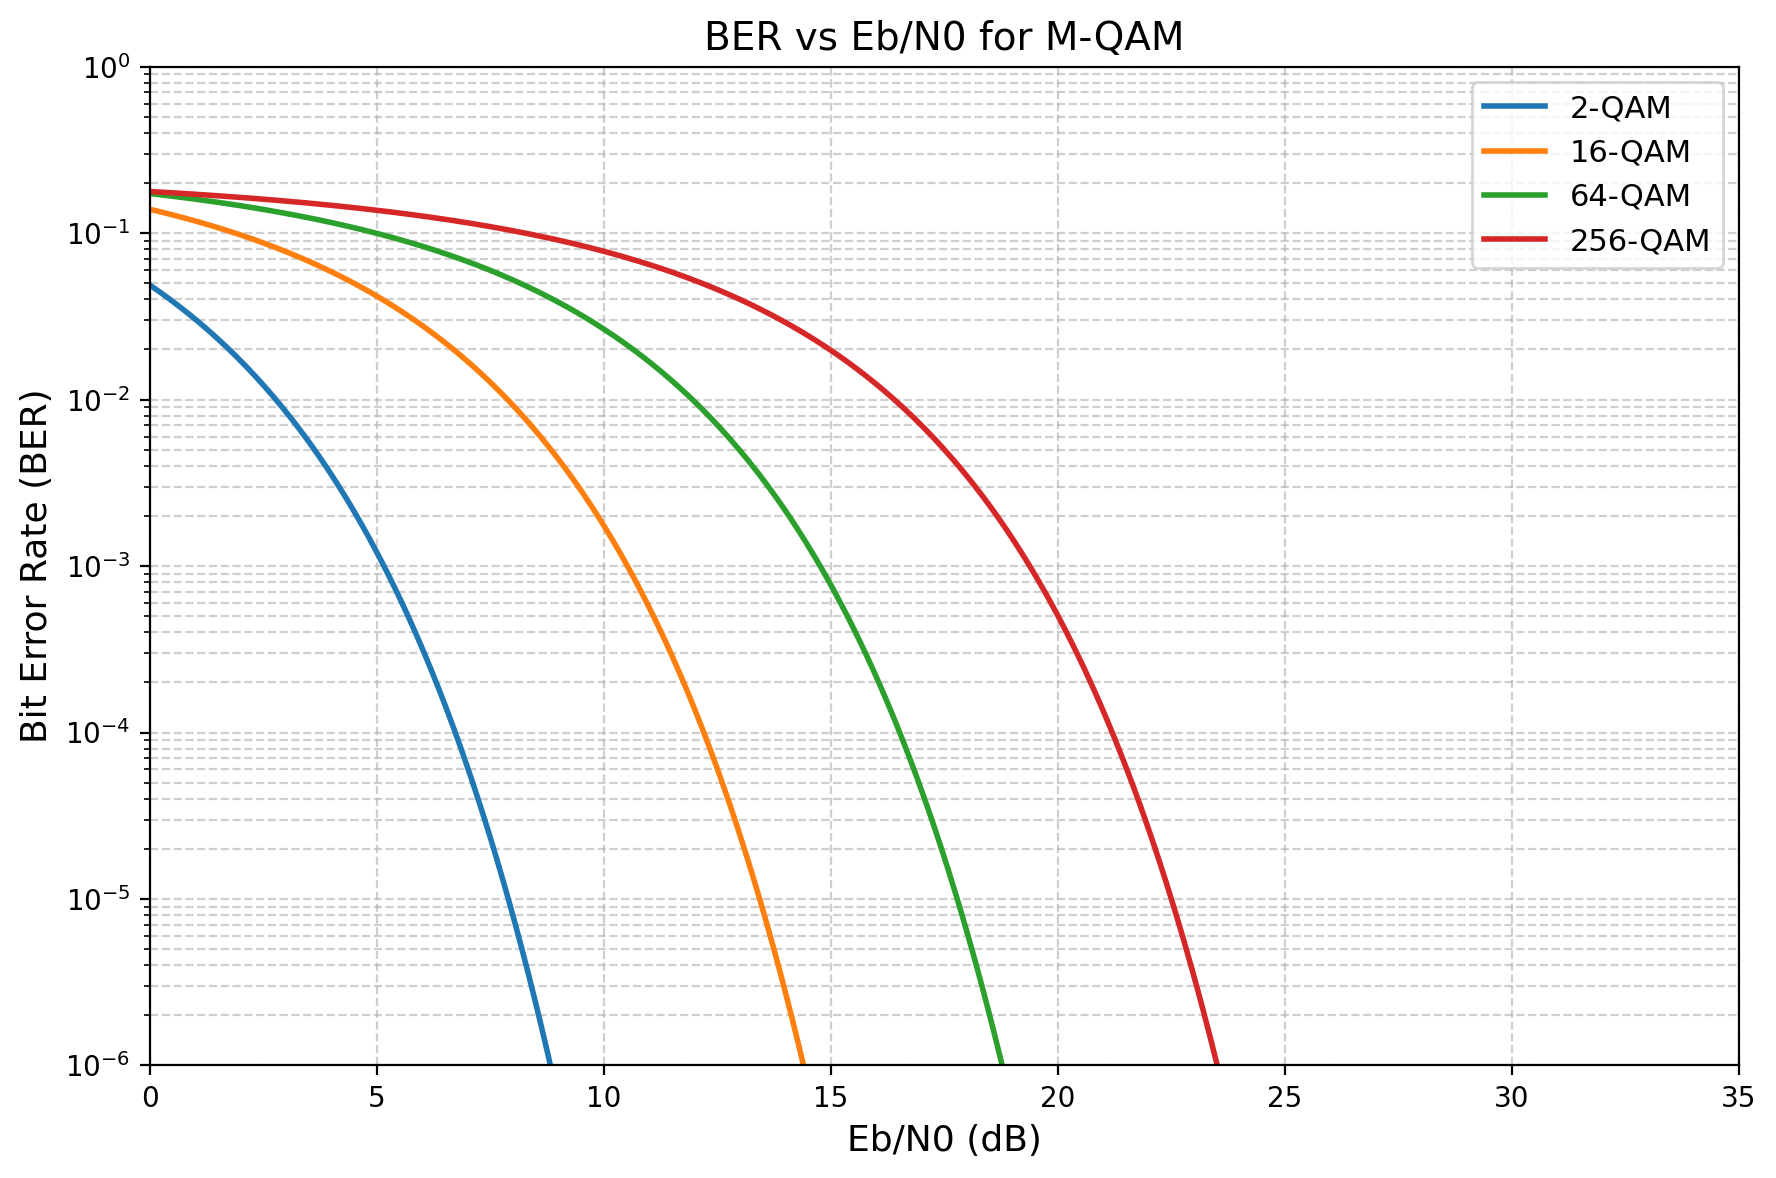
\includegraphics[width=\linewidth]{figures/ber_plot_1.png}
    \caption{Bit Error Rate plot of different QAM}
    \label{fig:BER_plot}
\end{figure}

The result is that two cells with identical PRB utilization can deliver very different data volumes depending on the network conditions experienced by their users, making SINR a fundamental determinant of cell capacity. Beyond its role in per user throughput, SINR is also an important indicator in network planning. Areas with consistently low SINR suggest poor coverage, which may indicate the need for additional infrastructure such as new base stations or upgrades to existing cells. In this way, signal quality metrics inform not only real-time scheduling decisions but also longer-term capacity planning. \\



\subsection{Resource Allocation and PRB Utilization}
\label{sec:resource_allocation}
In 5G NR and 4G LTE, the available frequency spectrum is organized into a two dimensional time frequency grid as seen in figure \ref{fig:prb_grid}. The frequency axis is 180khz wide divided into subcarriers spaced 15kHz apart \cite{ericsson5gnr}, while the time axis is divided into symbols. A Physical Resource Block (PRB) consists of 12 consecutive subcarriers in the frequency domain \cite{prb_grid}. This grid structure is a direct consequence of the OFDM waveform described in the previous section, where each subcarrier occupies a defined 15khz position in the frequency domain, without any cross talk. \\

\begin{figure}[h]
    \centering
    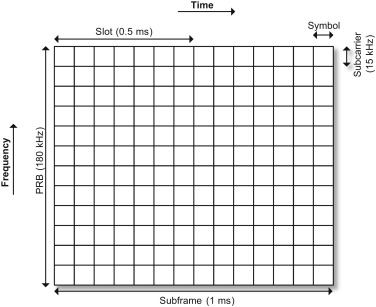
\includegraphics[width=\linewidth]{figures/prb_grid.jpg}
    \caption{PRB Time and Frequency resource grid}
    \label{fig:prb_grid}
\end{figure}

Each cell allocates its available PRBs between connected users through a scheduling process that runs every millisecond. During each scheduling interval, the base station evaluates all active users, their current data demand, and their radio conditions. Based on this information, PRBs are assigned to users according to a scheduling algorithm that balances throughput, fairness, and service requirements. \\

\subsubsection{Proportional Fair scheduling}
The most commonly used approach is Proportional Fair scheduling algorithm, it aims to achieve a trade off between maximizing total throughput and ensuring fairness among users with different radio conditions \cite{proportional-fair}. The key idea is to prioritize users who currently have good channel conditions relative to their past achieved throughput. \\

The PF scheduler computes a scheduling metric for each active user at scheduling time $t$: \\

\[
M_i(t) = \frac{T_{\text{inst},i}(t)}{\left[T_{\text{average},i}(t)\right]^a}
\]

where $T_{\text{inst},i}(t)$ is the instantaneous achievable throughput derived from channel quality indicator and the corresponding modulation and coding scheme, and $T_{\text{average},i}(t)$ is the long-term average throughput for user $i$, obtained using an exponentially weighted low-pass filter. The parameter $a$ controls the fairness--throughput trade-off and is typically set to 1 \cite{proportional-fair}. \\



%Each interval is divided into $X$ timeslots, as shown in Figure~\ref{fig:prb_grid}. These timeslots are assigned sequentially. After each assignment, the PF metric and throughput averages are updated before the next partition is scheduled. This allows multiple users to be served within a single interval, while still allowing a single user to receive multiple time slots within the same interval depending on their metric. \\

%At each scheduling step, the user with the highest metric is selected for resource allocation. The scheduling process is applied over a set of fixed scheduling resources rather than a single resource unit. \\

Each interval is divided into $N$ time slots, as shown in Figure~\ref{fig:prb_grid}. These time slots are assigned sequentially. After each assignment, the PF metric and throughput averages are updated before the next partition is scheduled. This allows multiple users to be served within a single interval, while still allowing a single user to receive multiple time slots within the same interval depending on their metric. \\

At each scheduling step, the user with the highest metric is selected for allocation of the current resource unit. This process is repeated over all fixed scheduling resources within the interval rather than resulting in a single user selection for the entire interval. \\

%%
%\subsubsection{PRB Utilization}
%Each cell allocates its available capacity between connected users by dividing the spectrum into small time frequency units called Physical Resource Blocks (PRBs). These blocks are the basic units used for data transmission. \\

%The base station runs a scheduling process every millisecond, during which it evaluates active users and their current data demand. Based on this information, Physical Resource Blocks (PRBs) are allocated according to each user's radio conditions and traffic requirements. Users with higher signal quality can transmit data more efficiently using higher-order modulation schemes, while users with lower signal quality require more PRBs to transmit the same amount of data. \\

\subsubsection{PRB Utilization}
PRB utilization measures the fraction of available resource blocks that are actively used during a reporting interval. It reflects the overall load of the cell by indicating how much of the available capacity is occupied at a given time, independent of how efficiently individual resource blocks are utilised. \\

High PRB utilization indicates a heavily loaded cell where most available resources are in use, while low utilization indicates available capacity. However, PRB utilization alone does not fully characterize cell performance, since it does not account for the efficiency with which each block is used. The relationship between PRB utilization and throughput provides a more complete picture of cell operating conditions, as illustrated in Figure \ref{fig:PRB_utilization}. \\
%PRB utilization measures the fraction of available resource blocks that are in use at a given time. It reflects how much of the cell’s capacity is being consumed. High PRB utilization indicates a heavily loaded cell, while low values indicate available capacity. \\

\begin{figure}[h]
    \centering
    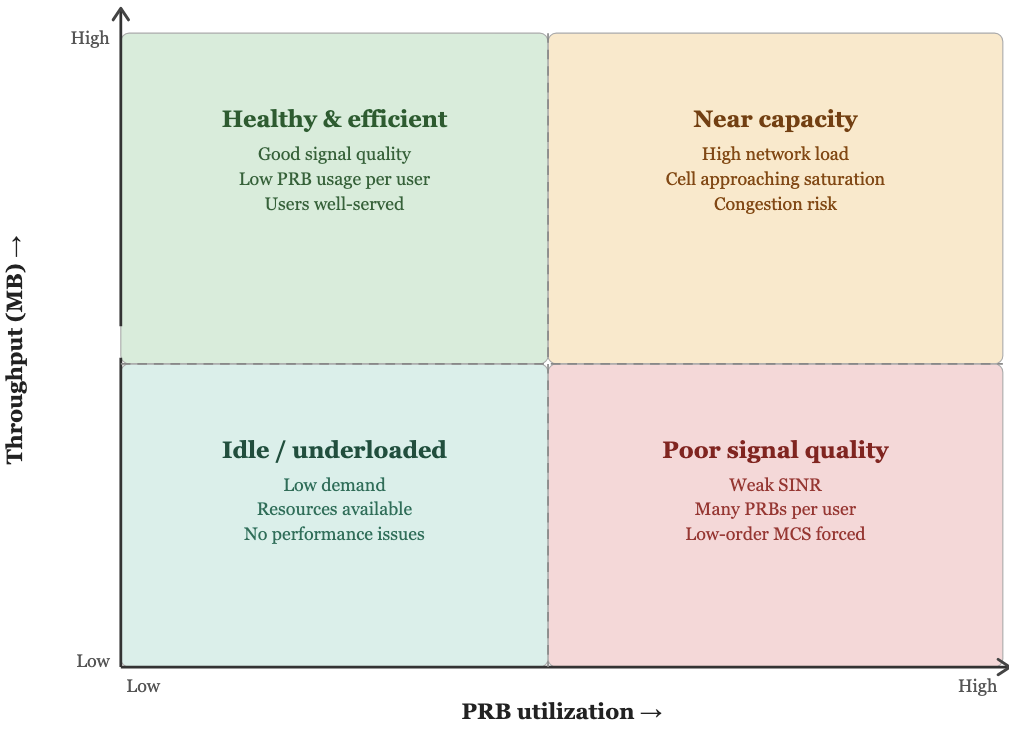
\includegraphics[width=\linewidth]{figures/prb_utilization.png}
    \caption{PRB utilization vs Throughput}
    \label{fig:PRB_utilization}
\end{figure}


Four general operating states can be identified from the relationship between throughput and PRB utilization as shown in figure \ref{fig:PRB_utilization}. Low PRB utilization combined with low throughput indicates an underloaded cell, where little traffic is being served and most resources remain idle. High PRB utilization combined with low throughput indicates inefficient resource use, typically caused by poor radio conditions that force the scheduler to allocate more PRBs per unit of data. High throughput combined with low PRB utilization indicates efficient operation under favorable radio conditions, where higher-order modulation allows more data to be carried by fewer blocks. Finally, high PRB utilization combined with high throughput indicates a heavily loaded cell operating close to its capacity limit, where resources are being used efficiently but congestion risk increases during periods of peak demand. \\

Among these states, high PRB utilization combined with low throughput represents the least efficient operating condition. It indicates that the cell is consuming a large share of its available radio resources while delivering relatively little user data, typically as a consequence of degraded signal quality across many connected users. \\


\subsection{Uplink and Downlink Traffic}

Traffic in cellular networks is directional. Downlink refers to data transmitted from the network to the user device, while uplink refers to data transmitted from the user device to the network. Applications such as video streaming, web browsing, and social media primarily generate downlink traffic, whereas uplink traffic typically consists of user-generated content, control signalling, and other lower-volume data transmissions. As a result, downlink traffic generally dominates in consumer mobile networks \cite{ericsson5gnr}. \\

This asymmetry is reflected in how cellular systems are designed. In Time Division Duplex (TDD) systems, uplink and downlink share the same frequency band but are separated in time \cite{ericsson5gnr}. The available resources are divided into time slots that are assigned to either uplink or downlink, allowing the network to adapt to traffic demand. In contrast, Frequency Division Duplex (FDD) systems use separate frequency bands for uplink and downlink, enabling simultaneous transmission in both directions. \\

In both cases, the overall resource allocation is typically biased heavily toward downlink traffic to reflect the dominant direction of data usage in mobile networks. \\

\subsection{Traffic Generation in Cellular Networks}
Cellular network traffic originates from individual user sessions, where a session referes to any period of data exchange between a users device and the network cell. These session can vary widely in terms of duration, data volume, uplink/downlink depeding on the application. Streaming videos generates a sustained high volume downlink session, while messaging generates short burst of low volume traffic, and audio calls generates a sustained low volume traffic. \\

At any given time, the traffic observed at the cell level is the sum of all active user sessions within that cell. This means that cell level traffic reflects the combined behavior of many independent users rather than a single transmission pattern. As a result, traffic at the network level follows human activity patterns. Users do not generate sessions uniformly over time, but instead concentrate activity around daily routines such as working hours and commuting. This leads to clear daily patterns, with high load during the day and lower activity during the night. Longer-term variations can also appear, including weekly differences between weekdays and weekends, as well as seasonal effects driven by travel and population movement. \\

Different geographical environments produce structurally distinct traffic patterns. Cells located near event venues such as stadiums and exhibition centers may experience long periods of low activity interrupted by short, sharp peaks triggered by external events. These series are non-stationary, since their statistical properties change abruptly during event windows. \\

Recreational cells serving destinations such as ski resorts, coastal regions, and holiday areas follow smoother and more regular seasonal cycles. These patterns are visible across months or years, with recurring peaks during specific periods. Traffic in these cells is typically not stable week to week, but exhibits seasonal cycles that repeat year to year. \\

Urban and commercial cells tend to exhibit a more stable traffic structure. Traffic is driven by regular human activity patterns such as work commutes and daily routines, producing strong and consistent daily and weekly cycles, including differences between weekdays and weekends. These series tend to be closer to stationarity compared to recreational or event-driven cells. \\

This user activity forms the basis of the measurements collected by the network. The base station continuously records and summarizes these events into cell level indicators, which are then reported as Performance Management (PM) counters at fixed time intervals. \\


\subsection{PM Counters}
Mobile network operators typically collect standardized measurements from their network cells using Performance Management (PM) counters. These are software counters embedded in the base station that continuously record network activity and report values at fixed time intervals, typically every 15 minutes or every hour, depending on the network configuration. \\

PM counters operate at the cell level, meaning that each counter value represents the combined activity of all users connected to a specific cell during the reporting interval. Typical counter categories include traffic volume counters, PRB utilization counters, unique user counters, and signal-to-noise ratio counters. Traffic measurements include both downlink and uplink counters, and most categories are reported as average and maximum values over the interval. \\

Traffic volume counters are typically implemented as cumulative sums of transmitted and received data bytes at the base station. These counters are incremented based on the actual number of successfully transmitted bits at the MAC or PDCP layer during scheduling. At the end of each reporting interval, the accumulated values are exported and reset or reported as deltas, and higher-level KPIs such as throughput are derived from these measurements. \\

%Because PM counters are based on fixed reporting intervals, they do not capture the instantaneous state of the network. Instead, they provide a statistical summary of network behavior over time. As a result, short bursts of network activity may be smoothed out and not fully reflected in the reported values. \\


